
%(BEGIN_QUESTION)
% Copyright 2012, Tony R. Kuphaldt, released under the Creative Commons Attribution License (v 1.0)
% This means you may do almost anything with this work of mine, so long as you give me proper credit

The stripper overhead temperature control system (loop \#21) works adequately, but not as good as it could.  In its present form, the temperature tends to be affected by variations in cooling water supply pressure, because this affects the differential pressure drop across control valve TV-21, and thus the flow rate through the cooling pipes in the upper section of the sour water stripping vessel:

$$\includegraphics[width=15.5cm]{i0007rx01.eps}$$

Modify this system for better control of stripper overhead temperature, using {\it cascade} control.

\vskip 20pt \vbox{\hrule \hbox{\strut \vrule{} {\bf Suggestions for Socratic discussion} \vrule} \hrule}

\begin{itemize}
\item{} Suppose you discovered that the stripper overhead temperature was also being affected by variations in the cooling water's {\it temperature} as well as by the cooling water's pressure.  Can you think of any control strategy that might help overcome this load variation?
\end{itemize}

\underbar{file i01696}
%(END_QUESTION)





%(BEGIN_ANSWER)


%(END_ANSWER)





%(BEGIN_NOTES)

Add a (cascaded) flow controller to TIC-21, with TIC-21 sending a setpoint to a flow controller (FIC-21), which monitors cooling water flow and throttles valve 21 (now named FV-21).










%INDEX% Control, strategies: cascade

%(END_NOTES)


